\chapter{\IfLanguageName{dutch}{Stand van zaken}{State of the art}}
\label{ch:stand-van-zaken}

% Tip: Begin elk hoofdstuk met een paragraaf inleiding die beschrijft hoe
% dit hoofdstuk past binnen het geheel van de bachelorproef. Geef in het
% bijzonder aan wat de link is met het vorige en volgende hoofdstuk.

% Pas na deze inleidende paragraaf komt de eerste sectiehoofding.

%Dit hoofdstuk bevat je literatuurstudie. De inhoud gaat verder op de inleiding, maar zal het onderwerp van de bachelorproef *diepgaand* uitspitten. De bedoeling is dat de lezer na lezing van dit hoofdstuk helemaal op de hoogte is van de huidige stand van zaken (state-of-the-art) in het onderzoeksdomein. Iemand die niet vertrouwd is met het onderwerp, weet nu voldoende om de rest van het verhaal te kunnen volgen, zonder dat die er nog andere informatie moet over opzoeken \autocite{Pollefliet2011}.
%
%Je verwijst bij elke bewering die je doet, vakterm die je introduceert, enz. naar je bronnen. In \LaTeX{} kan dat met het commando \texttt{$\backslash${textcite\{\}}} of \texttt{$\backslash${autocite\{\}}}. Als argument van het commando geef je de ``sleutel'' van een ``record'' in een bibliografische databank in het Bib\LaTeX{}-formaat (een tekstbestand). Als je expliciet naar de auteur verwijst in de zin, gebruik je \texttt{$\backslash${}textcite\{\}}.
%Soms wil je de auteur niet expliciet vernoemen, dan gebruik je \texttt{$\backslash${}autocite\{\}}. In de volgende paragraaf een voorbeeld van elk.
%
%\textcite{Knuth1998} schreef een van de standaardwerken over sorteer- en zoekalgoritmen. Experten zijn het erover eens dat cloud computing een interessante opportuniteit vormen, zowel voor gebruikers als voor dienstverleners op vlak van informatietechnologie~\autocite{Creeger2009}.
%
%\lipsum[7-20]

\section{AZ Glorieux omgeving}

\subsection{Omgeving}

Er zitten meer dan 1000 toestellen in het domein waar controle en overzicht voor nodig is. Het gaat om een ziekenhuis. Er is geen marge voor fouten en respons moet direct kunnen zijn.
Zowel Servers als client computers gebruiken Microsoft Windows besturingssysteem varianten. De softwarecatalogus is uitgebreid. Relevant is dat Office gebruikt wordt, ook Office 365.
Er ligt een grote nadruk op documentering. Hiervoor wordt SharePoint gebruikt.

\subsection{Toekomst}

Migratie naar Windows 10 is een lopend proces. Veel bedrijven doen dit en proberen dit te versnellen wegens de komende end-of-life status van Windows 7 \autocite{MicrosoftSupport2020}. Per case kan dit tijdrovend zijn om softwarecompatibiliteit te garanderen.
Verspreiding van nieuwe technologieën: interesse in het Power Platform, implementatie van Microsoft Teams, Intune wordt steeds meer gebruikt als aanvulling van SCCM (System Center Configuration Manager). Er worden steeds meer mobiele devices opgenomen in het domein.
Wat digitale transformatie betreft wordt sommige verouderde, huiseigen software vervangen. Concreet gaat het om tools gemaakt met Visual Basic.
Er wordt gestreefd naar een hogere mate van automatisatie. Het is wenselijk dat zoveel mogelijk software gedeployed kan worden vanuit SCCM.

\subsection{IT Asset Management}

Het onderzoek bevind zich in het domein van IT Asset Management. Enkele definities om dit begrip te verduidelijken.

\textcite{IAITAM} geeft een algemene definitie: `IT Asset Management is a set of business practices that incorporates IT assets across the business units within the organization. It joins the financial, inventory, contractual and risk management responsibilities to manage the overall life cycle of these assets including tactical and strategic decision making.`

\textcite{Gartner} stelt: `IT asset management (ITAM) provides an accurate account of technology asset lifecycle costs and risks to maximize the business value of technology strategy, architecture, funding, contractual and sourcing decisions.`

\textcite{Ivanti2018} reikt onderverdelingen aan. Er kan een onderscheid gemaakt worden tussen Fysieke, Digitale, Software, Mobile en Cloud IT Asset Management.
Een beschrijving voor de voor het onderzoek toepasbare categorie, de fysieke, geldt: 'The discovery and inventory of hardware including PCs, laptops, printers, copiers, and any other device used for IT and data management purposes'.

Er werd verwacht dat de IoT (Internet of Things) trend IT Asset Management programma's zal laten evolueren om met deze devices om te kunnen gaan. Dit betekend meer assets en meer asset types. Hier zijn voordelen mee verbonden: `Increased Operational Efficiency, Productivity Is Enhanced, Resources Are Used Efficiently, Better Checks for Safety and Compliance, Maintenance and Repair Automation` \autocite{Badnakhe2020}.

IT asset management oplossingen zijn vaak een aanvulling op het werken van SCCM. Een belangrijke functie van SCCM is het verschaffen van informatie. In sommige geevallen wordt functionaliteit van SCCM opgeroepen of zijn database geraadpleegd. Het is de moeite om meer informatie over SCCM te geven.

\textcite{Droogenbroot2016} beschrijft het als volgt: `System Center Configuration Manager, afgekort als SCCM of ConfigMgr, is een onderdeel van de Microsoft System Center Suite en staat in voor het beheer \& inventarisatie van pc's en servers. Daarenboven is het mogelijk toepassingen uit te rollen, software updates te installeren en compliance te controleren en op te lossen`.

De primaire functies zijn het creëren van computer images, massa deployment van images, distribueren van silent installaties van software applicaties, cross campus managen van software en natuurlijk inventarisatie en organisatie van eigen hardware en devices.

SCCM functioneert aan de hand van een aantal sleuteltechnologieën: PXE booting, de SCCM agent geïnstalleerd op client pc's die data voed aan SCCM en Task Sequences waarmee een hele reeks taken uitgevoerd kan worden. \autocite{Spitze2019}.

Eerder werd gesproken over de relatie tussen ITAM oplossingen en SCCM. Waar traditionele oplossingen een aanvulling of uitbreiding zijn op SCCM is LanReview eerder een vereenvoudiging. Het is toegespitst op inventarisatie en organisatie van eigen hardware en devices.

De reden dat SCCM zo verspreid is is omdat het gratis inbegrepen is in enterprice licensing van Microsoft. Het is bijvoorbeeld inbegrepen in Microsoft 365 licentie. \autocite{MicrosoftDocs2020}

\subsection{Databronnen}

Een overzicht van enkele databronnen die AZ Glorieux gebruikt. Deze zullen later in het onderzoek aan bod komen.

\begin{itemize}
    \item SQL Server
    \item Microsoft Excel en Access
    \item SharePoint
\end{itemize}

\section{LanReview}

\subsection{Visual Basic}

\begin{figure}[h!]
    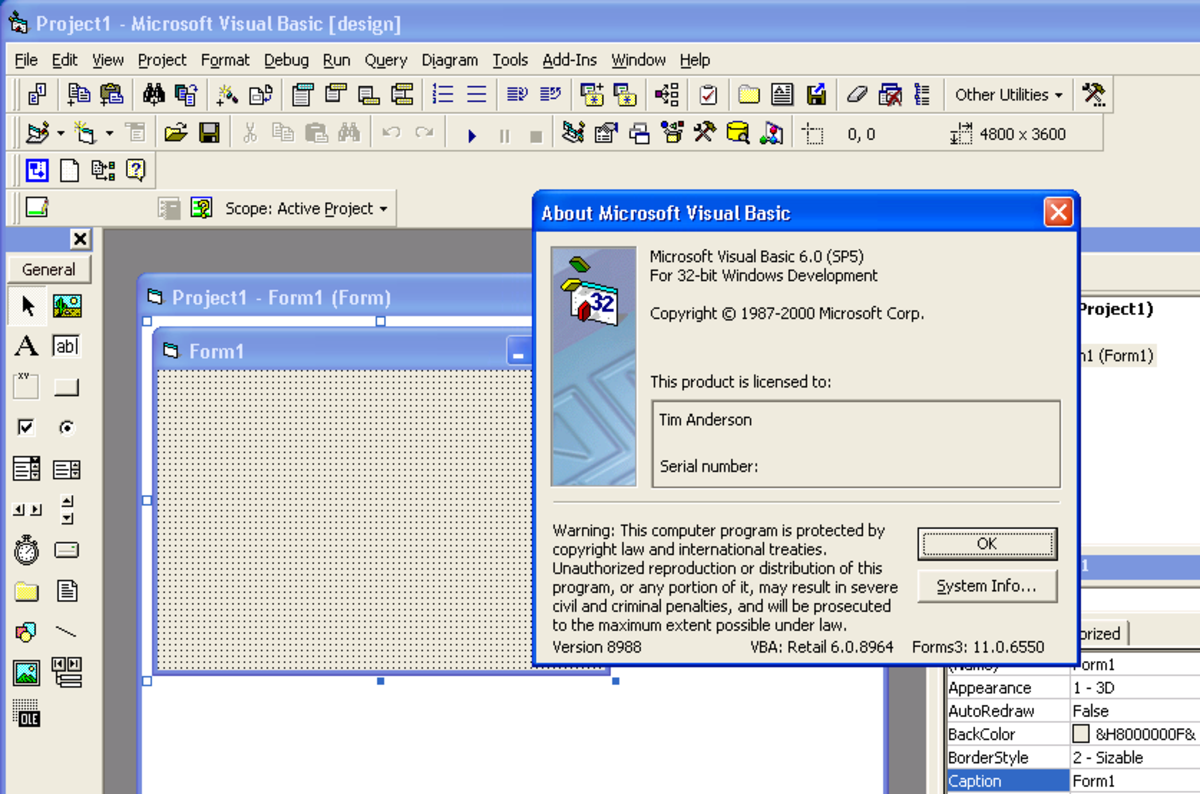
\includegraphics[width=\linewidth]{vb6.png}
    \caption{Voorbeeldweergave van de Visual Basic IDE \autocite{Speed2020}}
    \label{fig:vb6ide}
\end{figure}

LanReview werd gebouwd in Visual Basic (VB). Dit is een event-gedreven programmeertaal en omgeving van Microsoft waarmee programmeurs code kunnen aanpassen door drag-en-drop van objecten en door wijziging van hun gedrag en uiterlijk. VB komt van de BASIC programmeertaal. Het is een RAD (Rapid Application development) platform. Het werd voornamelijk gebruikt voor prototyping en als front-end voor databases. De laatste versie, Visual Basic 6.0, stamt van 1999.

Het grote voordeel is snelheid van ontwikkeling. Er zijn ook een aantal nadelen:
Het had veel geheugen nodig en was niet geschikt voor programma's die veel proceskracht nodig hadden, zoals games. Het is ook beperkt tot het Microsoft besturingssysteem.

\autocite{Rouse2019}

\subsubsection{Geschiedenis}

\begin{itemize}
    \item \textbf{1964}: BASIC geformuleerd door John Kemenu en Thomas Kurtz.
    \item \textbf{1987}: architect/programmeur Alan Cooper bedenkt voorloper van VB genaamd Tripod.
    \item \textbf{1988}: Bill Gates koopt de rechten voor Tripod.
    \item \textbf{1991}: Visual Basic 1.0 geïntroduceerd.
    \item \textbf{1998}: Visual Basic 6.0 geïntroduceerd.
    \item \textbf{2002}: .NET framework.
    \item \textbf{2008}: Einde extended support voor Visual Basic 6.0.
\end{itemize} \autocite{Grigonis2014}

\subsubsection{Vandaag}

Uitvoering van VB applicaties blijft ondersteund op moderne Windows versies. Het maken van nieuwe echter niet \autocite{MicrosoftDocs2018}. Niettegenstaande heeft men manieren gevonden om alsnog te installeren. \autocite{Brust2015}

Er is nog een kleine maar vocale groep aanhangers van VB. Dit komt omdat ze de officiële opvolger, Visual Basic .NET, niet waardig vonden voornamelijk omdat de afhankelijkheid van .NET een extra abstractielaag was. Voorbeelden hiervan zijn: % TODO: David Platt bron?
\begin{itemize}
    \item Visual Basic behoud blijft hoog. Opvallend aanhoudend succes voor een `dode` tool. \autocite{ISpliter2014}.
    \item Er werd een petitie gemaakt voor verdere ontwikkeling van VB. \autocite{2005}
    \item Er worden nog steeds applicaties mee ontwikkeld \autocite{Ippolito2018}.
\end{itemize}

\subsection{LanReview werking}

% TODO: afbeelding 1

LanReview houdt zijn informatie over assets in het domein bij in een Access databank. Deze informatie werd origineel geëxporteerd uit SCCM.
De applicatie heeft twee views: de primaire view is een filterbaar overzicht van devices. voor elke entry kan een meer gedetailleerde view opgeroepen waar alle datavelden te zien zijn.
Aan de hand van de filter functionaliteit worden SQL achtige queries gebouwd die dan uitgevoerd worden op de Acces databank.

LanReview is een belangrijke tool van de Helpdesk en wordt dagelijks gebruikt.

Vaak voorkomende use cases:
\begin{itemize}
    \item De pc overnemen van iemand in nood. Het is een startpunt voor remote management.
    \item Rapportage. Er kunnen voorgebouwde query's uitgevoerd worden op de data waarvan de resultaten onder andere naar Excel geëxporteerd kunnen worden.
    \item Filteren van de dataset. Bijvoorbeeld een overzicht van alle laptops van een belaad model tonen die nog steeds met Windows 7 werken.
    \item End of life beheer. Via markeringen is duidelijk of een device nog niet gebruikt wordt, in gebruik is of niet meer gebruikt wordt/in storage is.
\end{itemize}

% TODO: afbeelding 2 + uiteg datavelden

\section{Low Code}

\subsection{Basics}

De POC zal gebouwd worden met een low-code platform. Cloud services maken hier een deel van uit. Moderne low-code platformen zijn gecategoriseerd als PaaS (Platform as a Service). In geval van IaaS (infrastructure as a service) leeft de volledige infrastructuur in de cloud. PaaS kan gezien worden als een extra laag gebouwd bovenop IaaS waarmee applicatieontwikkelaars software kunnen programmeren in de cloud om later aan te kunnen bieden als SaaS (Software as a Service). Het is een tussenlaag gefocust op programmeurs. \autocite{Nucleus2017}

Definiëren van wat low-code zoal inhoud kan best begonnen worden met een formele definitie:\\
\textit{`It is an application platform that supports rapidapplication development, one-step deployment, execution and management using declarative,high-level programming abstractions, such as model-driven and metadata-based programminglanguages. They support the development of user interfaces, business logic and data services,and improve productivity at the expense of portability across vendors, as compared withconventional application platforms.`} \autocite{Vincent2019}

De bedoeling van low-code is om applicaties sneller te kunnen maken en ontwikkeling voor een grotere groep toegankelijk te maken. Typisch gezien wordt er een WYSIWYG (What You See Is What You Get) interface gebruikt waarin visuele componenten geconfigureerd worden via drag-and-drop. Vaak is er ondersteuning om aangepaste toe te voegen indien het platform bepaalde functionaliteit out of the box niet ondersteund. \autocite{Kissflow2018}

Low code is een software ontwikkelingsaanpak dat snellere oplevering van applicaties mogelijk maakt met minimaal manueel coderen. Dit werkt met visueel modeling in een grafische user interface om applicaties op te zetten en configureren. Hiermee slaat de ontwikkelaar de infrastructuur en her-implementatie van patronen die hun werk vertraagd en kunnen ze focussen op de unieke 10\% van een applicatie. \autocite{Revell2020}

Kissflow legt in zijn omschrijving nadruk op een grotere toegankelijkheid en Outsystems focust meer op het kunnen vermijden van herhalend werk.

Een low-code platform bestaat typisch uit volgende delen:
\begin{itemize}
    \item Een visuele IDE (Integrated Development Environment).
    \item Connectoren naar back-ends of services.
    \item App Lifecycle Management. Hiermee bedoelt geautomatiseerde tools voor build, debug, en deploy. Ook beheer van de app tijdens test, staging en productie.
\end{itemize} \autocite{Revell2020}

\subsubsection{low-code VS no-code}

Een no-code platform is een gespecialiseerde versie van een low-code platform waar men manuele aanpassingen zoveel mogelijk wil vermijden, al dan niet door het pre-builden van de nodige visuele componenten.

\textcite{Bloomberg2017} nuanceert de verschillen door te focussen op de bedoelde gebruiker:
\begin{itemize}
    \item low-code: Volgende generatie applicatie ontwikkeling dat het werk van professionele ontwikkelaars versneld en stroomlijnt.
    \item no-code: Self-service applicatie assembly voor business users die citizen developers worden.
\end{itemize}

\subsubsection{low-code development VS traditional software development}

% TODO: extra uitleg

\begin{landscape}
\begin{table}[]
    \begin{tabular}{@{}lll@{}}
        \toprule
        & \textbf{Traditional} & \textbf{Low Code} \\ \midrule
        1 & requirements bepalen & requirements bepalen \\
        2 & architectuur plannen & derde partij API's selecteren \\
        3 & selectie van back-end framework, bibliotheken, data-stores en API's & app workflow, data models en user interface tekenen in de visuele IDE \\
        4 & selectie van front-end framework & API's verbinden \\
        5 & keuze van deployment stack, opzetten van CI (Continuous Integration) en operatieplan creeren & indien nodig handgeschreven code toevoegen aan front-end of aanpassing van automatisch gegenereerde SQL queries \\
        6 & wireframes en prototypes maken & gebruikersacceptatietests \\
        7 & ui coderen in gekozen Javascript framework & deployment naar productie, hierna updates eenvoudig doorduwen \\
        8 & falende tests schrijven &  \\
        9 & modellen definieeren en koppelen aan data stores &  \\
        10 & business logic definieeren en coderen &  \\
        11 & views maken om JSON data te voorzien/ontvangen van en naar de front-end &  \\
        12 & implementeren van workflows &  \\
        13 & integreren van derde partij API's via gepubliceerde interface of support bibliotheek &  \\
        14 & herhalen tot tests slagen &  \\
        15 & testen voor security, performance, kwaliteit en gebruikersacceptatie &  \\
        16 & deploy, patch, monitor en updat tot levenseinde van de app &  \\ \bottomrule
    \end{tabular}
\end{table} \autocite{Revell2020}
\end{landscape} 

\subsubsection{Citizen developers}

De survey uitgevoerd door \textcite{McKendrick2017} geeft de volgende definitie:\\
\textit{`we define citizen developers as business users, not part of IT departments or contracted IT services, who build and use their own scripts, programs, algorithms, or interfaces designed to perform business functions or support business processes.`}

Er zijn enkele interessante statistieken uit voortgekomen:
\begin{itemize}
    \item Snelheid van applicatie delivery en delen van data/analytics worden aanzien als zwakke gebieden van IT support.
    \item 76\% van de respondenten zegt dat op z'n minst een deel van de gebruikte applicaties buiten het IT departement komen.
    \item 45\% van citizen development activiteiten worden tijdens de werkuren gedaan, de grootste motivatie hiervoor (42\%) is omdat het IT departement te traag is.
    \item In slechts 17\% van de gevallen duurt ontwikkeling van een citizen developer applicatie langer dan drie maand.
\end{itemize}

\subsubsection{Mythes}

Er bestaan enkele mythes rondom low-code:
\begin{itemize}
    \item Minder geschikt voor professionele gebruikers dan voor citizen developers \\
    $\rightarrow$ In praktijk wordt low-code vaker gebruikt door professionele ontwikkelaars.
    \item De nood om te programmeren wordt geëlimineerd \\
    $\rightarrow$ Het is vaak mogelijk om eenvoudigere applicaties te bouwen zonder code. Een typische business applicatie zal echter extra programmatie nodig hebben voor integratie met andere applicaties en databases, ook om aangepaste algoritmen te kunnen gebruiken. Deze use cases worden als extensies, externe programmatie of als scripts toegevoegd.
    \item low-code betekend kleine schaal \\
    $\rightarrow$ Er zijn genoeg praktijkvoorbeelden die dit tegenspreken. Neem bijvoorbeeld Sapphire HMS. \autocite{Bashar2017}
\end{itemize} \autocite{Richardson2016}

\subsection{Geschiedenis}

De oorsprong van low-code kan best bekeken worden vanuit het perspectief van de verranderingen in complexiteit en bruikbaarheid van programmeertalen doorheen de jaren. Er zijn enkele grote sprongen waarneembaar:
\begin{itemize}
    \item \textbf{Fortran}: niet intuïtief, nuttig voor wetenschappelijke en numerieke computing.
    \item \textbf{Cobol}: Focus buiten wetenschappers of wiskundigen. Syntax staat dichter bij Engels. Het hielp bij het vinden van oplossingen naar business taken.
    \item \textbf{C}: Geschreven met Engelse syntax. Bruikbaar in een grote variatie aan applicaties.
    \item \textbf{Internet}: Kwam door het internet en een groeiende populariteit van webapplicaties. Men is kleinere en eenvoudigere scripts beginnen gebruiken in plaats van complexe programmeertalen. Er was een focus op functie. Applicaties moeten aan een snellere pas ontwikkeld kunnen worden en talen moeten eenvoudig genoeg zijn om dit te ondersteunen.\\
    Een voorganger van low-code dat ook uit het internet is voortgekomen is het content management systeem. Wordpress is een bekend voorbeeld. Er zijn gelijkenissen in ideologie: het laat toe om de inhoud van een website aan te passen met een minimale hoeveelheid programmeren. Er worden modules gebruikt voor vaak voorkomende requirements. \autocite{Kissflow2018}
\end{itemize} \autocite{Kissflow2018a}

De ideologie achter low-code bestaat al een lange tijd. Er zijn cyclussen waar te nemen waarin de populariteit piekte. Een iteratie van 10 jaar geleden is 4gl (Fourth Generation Language). Een iteratie van 20 jaar geleden is RAD (Rapid Application Development). % TODO: welke bron?

Visuele en declaratieve development tools bestaan al decennia maar elke iteratie zijn er minder technische skills nodig om complexere business apps te kunnen maken die ook kunnen omgaan met moderne scenario's. Moderne low-code platformen overstijgen de limieten van op een aantal manieren: \\
\textbf{Ze zijn meer `open`.} Vaak worden platform API's en adapters ondersteund. Soms is mogelijk om Java of .NET code te genereren als maatregel tegen vendor lock-in. Sommige platformen gebruiken zelf open source development frameworks zoals AngularJS, Apache Cordova en Bootstrap.\\
\textbf{De platformen zelf zijn `completer`.} De vorige generaties waren eerder tools. Moderne low-code platformen ondersteunen de volledige applicatie levenscyclus.\\
\textbf{Betere integratiemogelijkheden.} De meeste low-code platformen laten laten toegang tot tot externe data toe. Vaak zijn er API's voor integratie mer externe applicatie modules. 

\autocite{Richardson2016}

\subsection{Nood / Voordelen}

\begin{figure}[h!]
    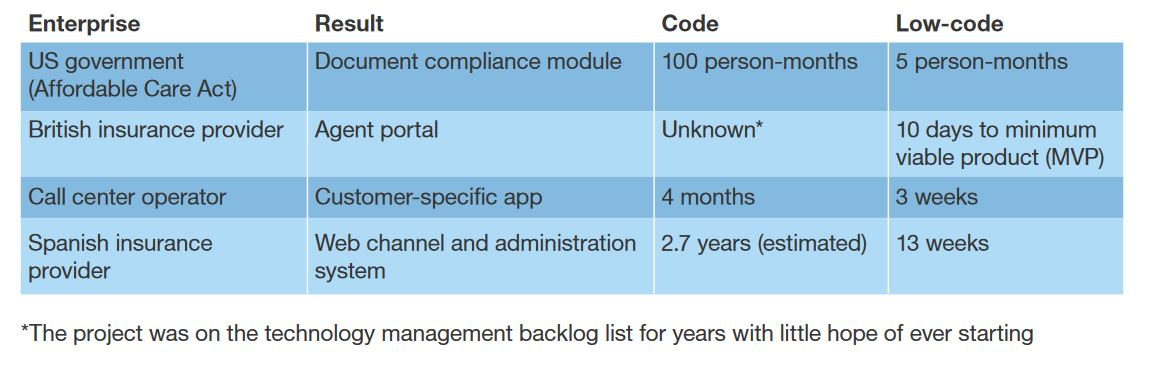
\includegraphics[width=\linewidth]{lowcode-time.JPG}
    \caption{Vergelijking van doorlooptijd \autocite{Richardson2016}}
    \label{fig:tijdverschil}
\end{figure}

Het verkooppunt van low-code is hogere snelheid van applicatieontwikkeling. Naast deze snelheid zijn er nog andere voordelen:
\begin{itemize}
    \item Betere collaboratie tussen business en IT: Business shareholders zien hun visie sneller vorm nemen en kunnen rappe aanpassingen doorvoeren. Business regels zijn geïntegreerd in het bouwen van de applicatie.
    \item Focus op functionaliteit: Er wordt geen tijd verspild met schrijven van herhalende code.
    \item Transparante deployment: Er zijn geen aanpassingen meer nodig om verschillende architecturen te kunnen ondersteunen.
    \item Lange termijn gebruik: Apps zijn eenvoudig aan te passen.
    \item Enkele code base: Minder ruimte voor fouten en de code base wordt ook niet vervuild met tijd.
\end{itemize} \autocite{Schetsen2016}

Markt leidende platformen hebben de volgende eigenschappen:
\begin{itemize}
    \item Eenvoudige visuele configuratie
    \item Veel integratie opties.
    \item Mobile compatibel.
    \item Schaalbaar.
    \item Support over de volledige app levenscyclus.
\end{itemize} \autocite{Kissflow2018}

Het perspectief van de klant, welke waardepropositie er is. Dit is duidelijker als er eerst naar de omgeving gekeken wordt. Bedrijven moeten steeds meer kunnen omgaan met disruptieve innovatie en wijzigend klantgedrag. De vraag naar applicaties is vaak groter dan wat geleverd kan worden. Er zijn strategieën om hier mee om te proberen gaan zoals outsourcing, hackathons of voorgebouwde softwareoplossingen. Low code is een nieuwe manier om er mee om te kunnen gaan. De waardepropositie voor de business en het tech management is:
\begin{itemize}
    \item Apps visueel configureren in plaats van manueel te coderen. Ontwikkeling kan zo mogelijk met een factor 5 tot 10 versneld worden.
    \item Echte requirements en zo echte waarden vinden. Met low-code kunnen snel minimum viable products gebouwd worden om klantenideeën te toetsen.
    \item Live-trial van business ideeën tegen lage of onbestaande kost. Ideen kunnen snel omgezet worden in een werkend prototype dat gedeployed en getest kan worden op de markt.
    \item Werkende prototypes kunnen in vijf minuten omgezet worden in productie apps. Het komt niet voor dat een app opnieuw gebouwd moet worden om een hoger volume of hogere diversiteit van gebruikers aan te kunnen.
    \item Meer development talent mogelijk. Developers zonder formele achtergrond kunnen door het visuele aspect nu ook business applicaties bouwen.
\end{itemize} \autocite{Richardson2016}

\subsubsection{Digitale transformatie}

Digitale transformatie is het proces van het gebruik van digitale technologie om nieuwe - of bestaande - business processen, cultuur en klantenexperience te maken als antwoord op veranderende business en markt requirements. Het is kortweg opnieuw bedenken van business in het digitale tijdperk. \autocite{Salesforce}
Digitale transformatie wordt steeds belangrijker als arena waarin business een voordeel kan krijgen op de competitie. Low-code wordt hierbij aanzien als een krachtig wapen in dit proces.

\subsection{Kritiek / Nadelen}

Er zijn een aantal valkuilen waar rekening mee gehouden moeten worden bij de keuze van een platform. De inzetting kan falen en het gewenste resultaat kan uitblijven als de klant geen concreet plan heeft over hoe low-code in te werken in zijn portfolio. Het is ook aangeraden om op te passen indien er een kleinere vendor gekozen wordt. Het is een veranderende markt en deze hebben een lagere stabiliteit. \autocite{Richardson2016}

Een mening is dat de business kant zijn mentaliteit ten opzicht van IT moet aanpassen. Al decennia probeert met de nood van programmeren terug te drijven en in functie hiervan worden tools gemaakt. Bedrijven zijn hiertoe aangetrokken om kosten te kunnen besparen. Maar de achterliggende kennis blijft nodig, vooral als er iets fout gaat. Niet alles kan visueel gedaan worden. Development talent blijft dus nog nodig. De aanpassing in mindset die gevraagd wordt is dat business het feit aanvaard dat software ontwikkeling duur en moeilijk is en dat er geen schortcuts voor zijn. \autocite{Reselman2018}

Er kan gesteld worden dan niet elk low-code platform daadwerkelijk 'low-code' is en dat men hiervoor moet oppassen:
\begin{itemize}
    \item \textbf{NIET} low-code: Het platform genereert statisch code en verstopt deze effectief voor de gebruiker. De code is niet flexibel en schaalt niet. Dit staat digitale transformatie in de weg en verhoogt technical debt in plaats van dit te verlagen.
    \item \textbf{WEL} low-code: Het platform is flexibel en schaalbaar. De volledige levenscyclus van de app moet ondersteund worden. Achterliggend wordt een model gedreven architectuur gehanteerd. De flexibiliteit komt doordat de model componenten geabstraheerd worden naar XML. De applicatie kan ook makkelijker gewijzigd worden en is eenvoudig schaalbaar.
\end{itemize} \autocite{Shiah2018}

\subsubsection{Shadow IT}

Gebruik van no-code tools in de handen van citizen developers kan mogelijk leiden tot shadow IT. Dit komt voor wanneer de IT organisatie te traag en proces-gebonden is om snel genoeg te kunnen reageren op de noden van business en business users buiten IT gaan om zelf een app bouwen. Zonder overzicht en coördinatie kunnen security kwetsbaarheden en compliance overtredingen verspreiden. Deze apps kunnen ook redundant en van lage kwaliteit zijn. \autocite{Bloomberg2017}

\subsection{Markt en Evolutie}

\begin{figure}[h!]
    \centering
    \begin{subfigure}[b]{0.4\linewidth}
        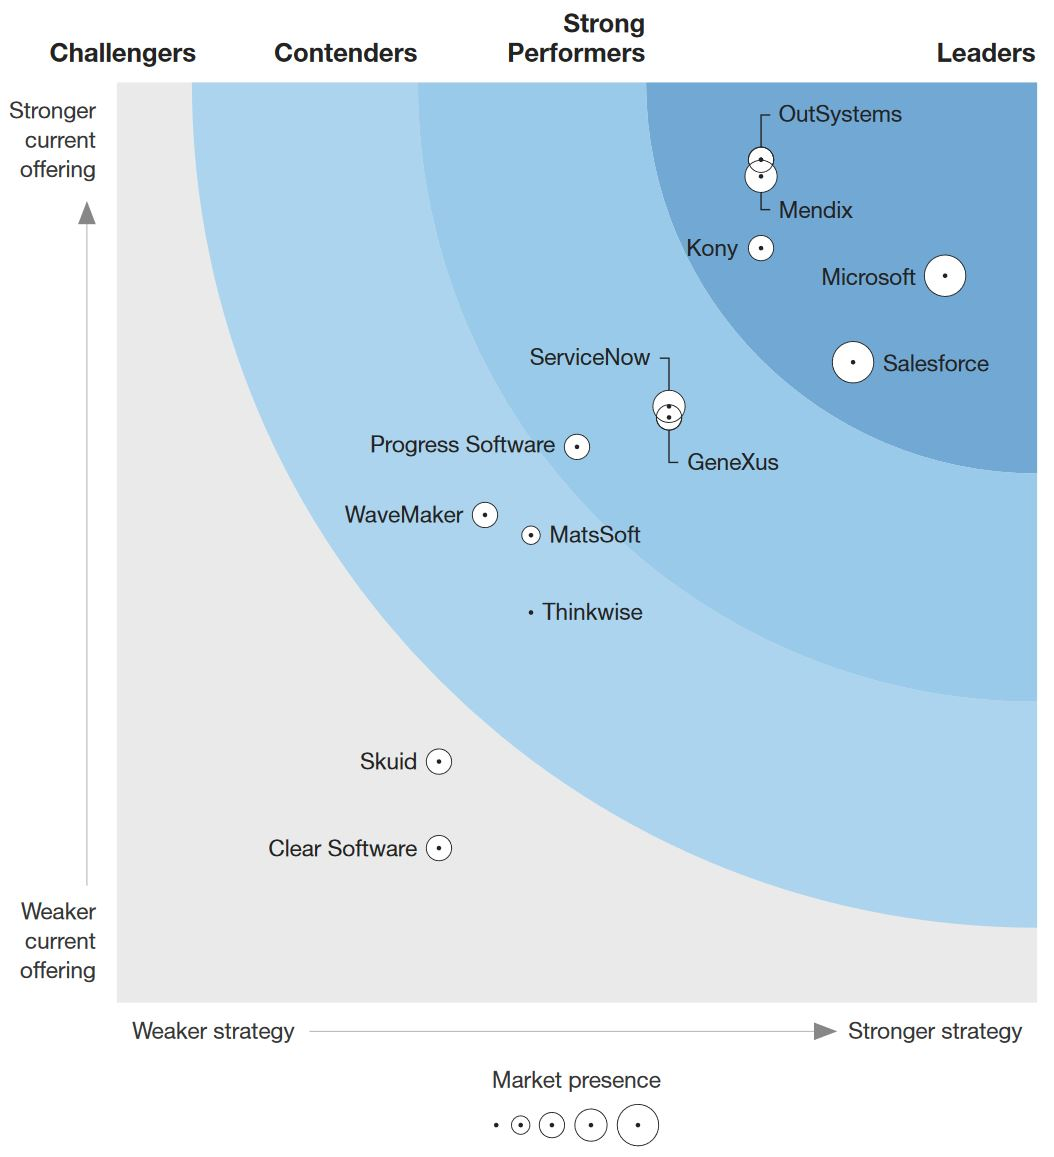
\includegraphics[width=\linewidth]{forrester-wave.JPG}
        \caption{Forrester Wave \autocite{Rymer2019}}
    \end{subfigure}
    \begin{subfigure}[b]{0.4\linewidth}
        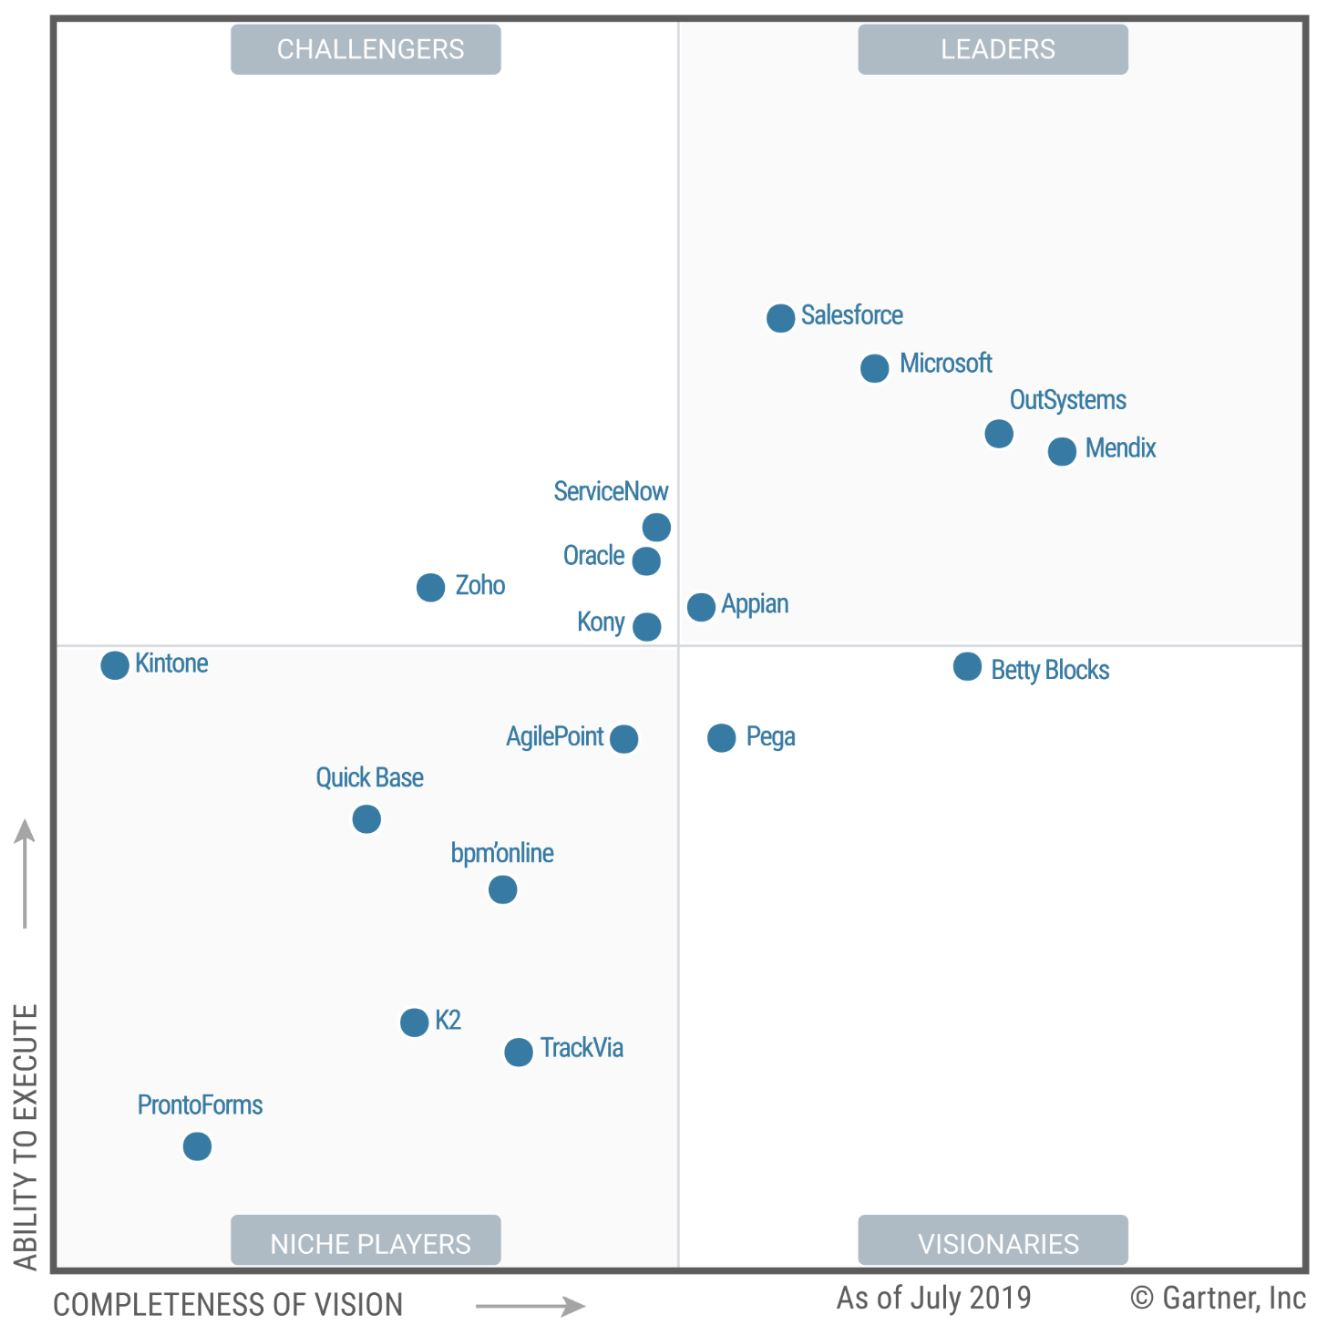
\includegraphics[width=\linewidth]{gartner-quadrant.JPG}
        \caption{Gartner Magic Quadrant \autocite{Vincent2019}}
    \end{subfigure}
    % \caption{overkoepelende caption}
    \label{fig:quadwave}
\end{figure}

Het business model van low code platformen is anders dan dat van traditionele platformen zoals Java of .NET. Er wordt uitgegaan van geleverde business waarde in plaats van beloofde. Zo zijn veel platformen gratis of tegen lage kost toegankelijk. Inkomst wordt gegenereerd uit benoemde gebruikers, gedeployde apps en nodige capaciteit. \autocite{Richardson2016}

Wat betreft marktsegmentatie heeft er zicht op relatief korte tijd veel evolutie voorgedaan. Er kunnen drie grote stappen onderscheiden worden:
\begin{enumerate}
    \item 5 marktsegmenten waarvan de grootste general purpose is. Het doel is grote variatie aan web en mobiele applicaties kunnen bouwen. Declaratieve tooling gebruikt met aandacht voor creatie, integratie, deployment life-cycle management en distributie van applicaties. Hiernaast waren ook nog segmenten voor process, database, request-handling en mobiele apps.
    \item Samensmelting naar general purpose % TODO: bron
    \item Splitsing om te focussen op gebruiker. Business user of professionele ontwikkelaars. % TODO: bron
\end{enumerate}

Er worden een aantal marktontwikkelingen verwacht:
\begin{itemize}
    \item \textbf{Consolidatie}. Grote verkopers zullen low-code platformen overnemen.
    \item \textbf{Marktsegment veranderingen}. Low code for mobile verdwijnt en low-code for process groeit naar general purpose segment.
    \item De volgende innovatie zal \textbf{ondersteuning voor IoT} zijn.
\end{itemize} \autocite{Richardson2016}

\textcite{Rymer2019} identificeert 5 marktleiders. Opvallend is dat Microsoft in een korte periode naar een leidingspositie is gesprongen. De bevindingen van \textcite{Richardson2016} sluiten hierbij aan.

\begin{table}[]
    \begin{tabular}{|l|l|l|l|l|l|}
        \hline
        \textbf{Forrester} & Salesforce & Microsoft & Mendix     & Outsystems & Kony   \\ \hline
        \textbf{Gartner}   & Salesforce & Microsoft & Outsystems & Mendix     & Appian \\ \hline
    \end{tabular}
\end{table}

Prospecten voor de komende vijf jaar:
\begin{itemize}
    \item Tegen 2024 zal drie vierde van grot enterprises ten minste vier low code development platformen gerbruiken voor zowel IT app development en citizen development initiatieven.
    \item tegen 2024 zal low-code applicatie development verantwoordelijk zijn voor 65\% van totale applicatie ontwikkeling activiteit.
\end{itemize} \autocite{Vincent2019}

De verschuiving van traditionele naar low-code software ontwikkeling is terug te vinden in huidige jobaanbiedingen\footnote{https://stagebank-hbo-ict.irp.nl/internships/12543/}\footnote{https://stagebank-hbo-ict.irp.nl/internships/12378/}.

Er wordt verwacht dat de low-code markt tegen 2022 21 biljoen dollar waard zal zijn. Er wordt ook voorspeld dat de jaarlijkse groei van 50\% zich verder zal zetten. \autocite{Rymer2018}

\begin{figure}[h!]
    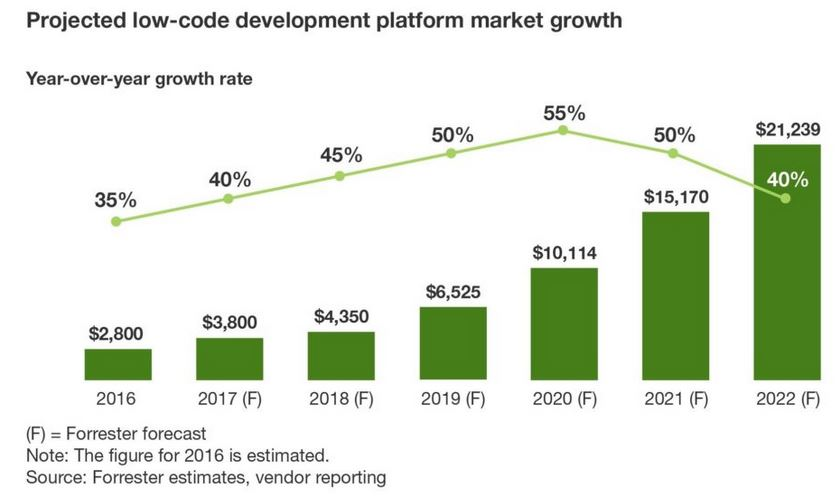
\includegraphics[width=\linewidth]{forrester-markt-evolutie.JPG}
    \caption{Forrester voorspelde markt evolutie \autocite{Rymer2018}}
    \label{fig:marktevolutie}
\end{figure}

\subsection{Voorgaand onderzoek}

Er is al redelijk wat praktisch onderzoek gevoerd die het potentieel van low-code illustreert maar het grootste succesverhaal is dat van Sapphire HMS. Dit is een low-code applicatie binnen gezondheidszorg. Koeweit had nood aan een nieuw ziekenhuis managementsysteem. Na initieel falen om iets manueel te bouwen werd gekeken naar low-code platformen en was het mogelijk om de eerste implementatie na 6 maanden in gebruik te nemen. \autocite{Bashar2017}

\subsubsection{Proof of Concepts}

Er werd onderzoek gedaan naar de mogelijke meerwaarde van low-code in een KMO omgeving. Uit vier marktleidende platformen werd Outsystems gekozen. Er werden POC's voor vaak voorkomende scenario's mee opgesteld. De bouw we snel, eenvoudig en er waren geen obstructies. De nodige investering van tijd, geld en kennis was beperkt \autocite{Devloo2018}.

Microsoft Power Apps werd gebruikt om enkele administratieve bedrijfsprocessen van verhuisbedrijf De Borger te optimaliseren. Het resultaat werd effectief in gebruik genomen de tijdswinst sinds implementatie werd berekend en significant bevonden. De prijs was aanvaardbaar. Er was slechts 5 euro per maand nodig om een aangepaste connector te kunnen gebruiken. \autocite{Spriet2019}

In een ander geval werd Power Apps gebruikt om een mobiele reporting applicatie te maken voor gebruik in de bouwsector. Er werd ok gebruik gemaakt van Power Automate om afbeeldingen te verwerken en SharePoint om deze op te slaan. \autocite{Aho2018}

Binnen de gezondheidszorg werd er een case study gedaan naar hoe onderzoeksdata verzameld kon worden door gebruik van een low-code platform. Er werd voor Mendix gekozen. De veiligheid van het platform werd als goed bevonden, relevant privacywetten waren gerespecteerd en authenticatie werd ondersteund en was eenvoudig te implementeren. Er werd verhoogde productiviteit waargenomen. \autocite{Totterdale2018}

\subsubsection{Enquetes}

Er werd onderzocht of het mogelijk zou zijn om een EHR (electronic Health Records) systeem te bouwen met low-code om te gebruiken op nationaal niveau. Dit was naar aanleiding van het Akson planningsproject voor een nieuw EHR systeem in Noorwegen. Er werden kwalitatieve interviews afgenomen bij mensen met expertise in low-code en mensen met kennis van het Akson project. \autocite{Ness2019}

Low-code en traditionele softwareontwikkeling werden met elkaar vergeleken aan de hand van interviews met medewerkers bij een Fins software consultancy bedrijf. Er kon besloten worden dat zowel de medewerkers als de klanten oplossingen gebouwd met low-code verkozen. \autocite{Virta2018}

\section{Microsoft Power Platform: Power Apps}

\subsection{Wat?}

\begin{figure}[h!]
    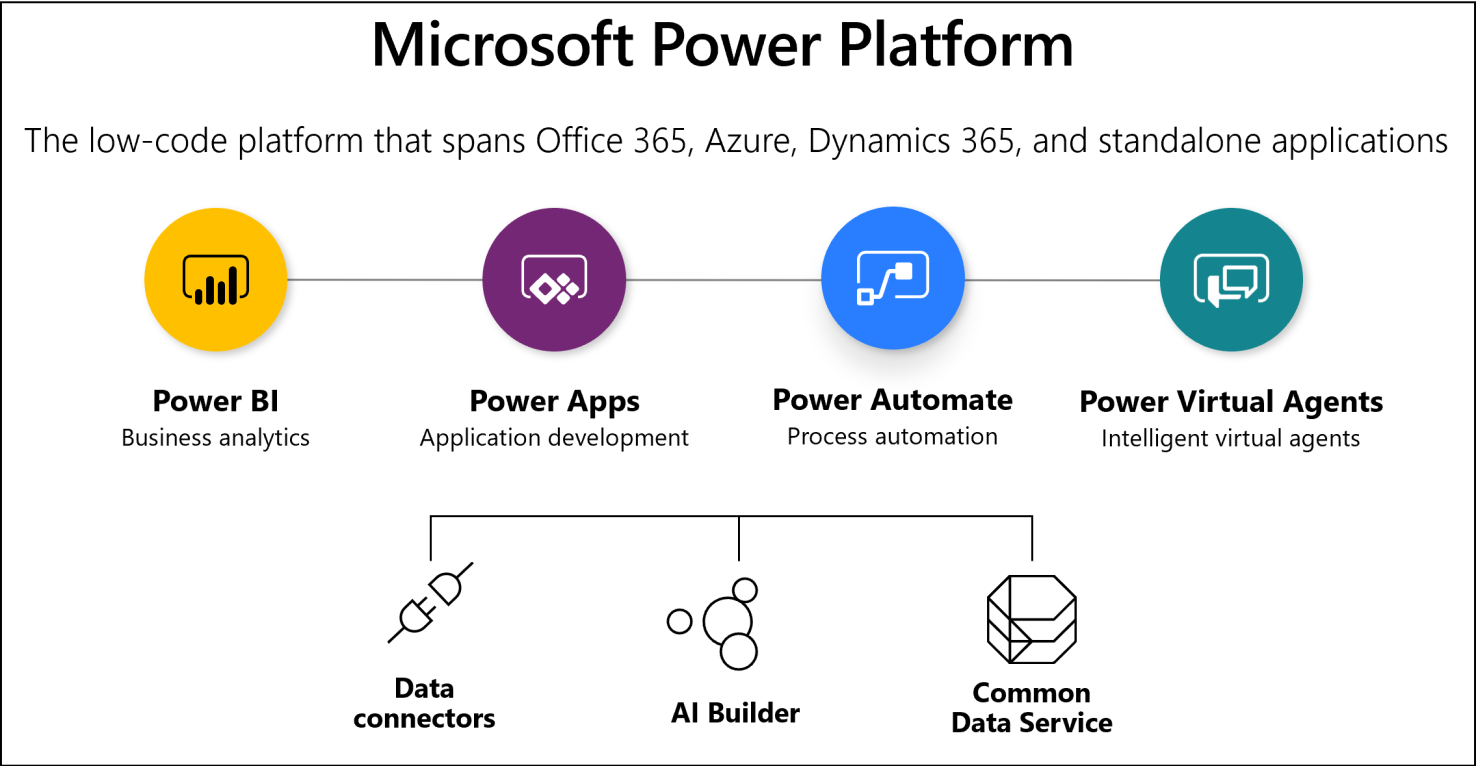
\includegraphics[width=\linewidth]{platform.png}
    \caption{Overzicht Microsoft Power Platform \autocite{MicrosoftDocs2019a}}
    \label{fig:mspowerplatform}
\end{figure}

Power Apps is een suite met apps, services en connectors. Het is een gegevensplatform die een snelle ontwikkelomgeving biedt om aangepaste apps te bouwen voor zakelijke behoeften. Men kan verbinden met zakelijke gegevens die zijn opgeslagen ofwel in het onderliggend gegevensplatform (Common Data Services), ofwel in de verschillende online en on-premises gegevensbronnen (SharePoint, Excel, Office 365, Dynamics 365, SQL Server enzovoort). De apps hebben een responsief ontwerp en kunnen zowel in een browser of op mobiele apparaten (telefoon of tablet) uitgevoerd worden. \autocite{MicrosoftDocs2019}

\subsection{Drie soorten apps}

\subsubsection{Canvas apps}

Populairste en meest toegankelijke variant. Er is een focus op het grafische. Zo worden de apps via een WYSIWYG (What You See Is What You Get) manier gebouwd. Daarmee is er volledige controle over de User Experience. Er is zowel tablet als mobile layout mogelijk. Men kan verder connecteren met meerdere data bronnen. Het resultaat zijn taak- en rol gebaseerde apps. \autocite{PragmaticWorks2019}

\subsubsection{Model Driven apps}

In tegenstelling tot Canvas apps begint men hier bij het data model. Deze data moet ook in de CDS leven. Het doel is meestal om complexe business processen te visualiseren. Het resultaat zijn dan ook end-to-end business applicaties. \autocite{PragmaticWorks2019}

\subsubsection{Portals}

Waar Canvas en Model apps naar binnen, naar internet business gebruikers gericht is, is Portals naar buiten gericht. Met portals kunnen extern gefocuste websites gebouwd worden waarmee gebruikers buiten de organisatie kunnen inloggen met een variëteit aan identiteiten, data in de Common Data Services kunnen bekijken of inhoud anoniem browsen. Er zijn zowel interne als externe gebruikers mogelijk. \autocite{MicrosoftDocs2020a}

\subsection{Belangrijke Onderdelen}

\subsubsection{Common Data Service}

Met de common data service kan data gebruikt door business applicaties opgeslagen en gemanaged worden. Data wordt opgeslagen binnen een set entiteiten. Een entiteit is een set van records om data op te slaan, zoals tables data opslaan in een database. Er zijn standaard entiteiten aanwezig voor typische scenario's, er kunnen ook aangepaste entiteiten gemaakt worden. Data wordt opgeslagen in de cloud. Er is ook logica en validatie mogelijk in de vorm van berekende velden, business regels, workflows en business process flows. Het 'common' aspect: De databronnen zijn gelinkt, als data in de ene bron aangepast wordt zal de relevante data in de andere bron automatisch aangepast worden. \autocite{MicrosoftDocs2019a}

\subsubsection{Connectors}

Data die een app nodig heeft is opgeslagen in een data bron, deze data naar de app brengen wordt gedaan door er een connectie voor te maken. Deze connectie heft een specifieke connector nodig om te kunnen praten met de data bron. Power Apps heeft connectors voor enerzijds populaire services en anderzijds on-premises data opslag. \\
Een connector kan in de app zelf dan ofwel tabellen of acties voorzien.

Een overzicht van de belangrijkste connectors:
\begin{itemize}
    \item Common Data Service
    \item Cloud storage: Voor elke grote provider. Bijvoorbeeld Google Drive of OneDrive.
    \item Excel: om excel data te kunnen tonen in de app. Requirements zijn dat de data geformatteerd moet worden als tabel en het bestand in de Cloud opgeslagen moet zijn.
    \item Office 365 (Outlook): Onder andere mogelijk om mails te tonen, versturen, beantwoorden of te deleten.
    \item Office 365 (Users): Toegang tot de gebruikersprofielen in de organisatie.
    \item Oracle DB
    \item Power BI
    \item SharePoint
    \item SQL Server
    \item Twitter
\end{itemize} \autocite{MicrosoftDocs2020b}

\textbf{On-premises data gateway}: Om on-premises data bronnen te kunnen gebruiken binnen een Power is moet een er een data gateway voor aanwezig zijn. Dit is een soort van brug tussen de on-premises data en de Microsoft cloud services die veilige data overdracht garandeert. \autocite{MicrosoftDocs2019b}

\subsubsection{Formules}

\begin{figure}[h!]
    
\includegraphics[width=\linewidth]{formula-bar.JPG}
    \caption{Overzicht van de formulebalk \autocite{MicrosoftDocs2019c}}
    \label{fig:msformulebalk}
\end{figure}

Logica en werken met gegevens is mogelijk met Excel-achtige expressies.\\
In Excel worden formules gebruikt om cellen te vullen of grafieken en tabellen te maken. In Power Apps worden vergelijkbare formules gebruikt om besturingselementen in plaats van cellen te configureren. Concreet ook om om te gaan met user input. De granulariteit is: een app bestaat uit UI controls $\rightarrow$ elke control heeft properties $\rightarrow$ per property kunnen formule(s) ingesteld worden. \autocite{MicrosoftDocs2019c}

\subsubsection{Overig}

Nadat werk aan een app opgeslagen is moet deze gepubliceerd worden om bruikbaar te zijn voro ander leden van ed organisatie.

Versiebeheer is beperkt aanwezig. Er kan eenvoudig teruggegaan worden naar eerder gepubliceerde versies van een app.

UI Tests zijn mogelijk met de Test Studio maar op moment van schrijven is dit nog experimenteel. Power Apps Test Studio is een low-code oplossing om tests te schrijven, organiseren en automatiseren voor canvas apps. In de Test Studio kunnen tests geschreven worden via Power Apps expressies of door gebruik van een recorder om app interactie op te slaan en expressies automatisch te genereren. De tests kunnen hierna teruggespeeld worden binnen de Test Studio om app functionaliteit te valideren. \\ 
Gebruikte concepten en terminologie komen overeen met gangbare testing frameworks zoals bijvoorbeeld JUnit voor Java. \\
Meer uitleg aan de hand van deze terminologie. 
\begin{itemize}
    \item \textbf{Test Cases}: Test cases bestaan uit een serie instructies of acties genaamd test stappen. Test cases worden utigevoerd om te controleren of apps of specifieke features in de app werken zoals verwacht. Deze test stapen zijn gescreven in de Power Apps expressie taal.
    \item \textbf{Test Suites}: Gebruikt om test cases samen te froeperen.
    \item \textbf{Test Assertions}: gebruikt om te valideren of het verwacht resultaat overeen komt met het verkregen resultaat. Evalueert naar true of false.
\end{itemize}
\autocite{MicrosoftDocs2019d}

Tot op heden werd is er nog geen IT Asset Management app gebouwd in Power Apps die als template terug te vinden is. Wel bestaat er een Asset checkout app. Dit staat er dicht genoeg bij. \autocite{Meganathan2019}

\subsection{IDE overzicht}

De onderdelen van Power Apps Studio uitgelicht volgens Figuur \ref{fig:pastudio}:
\begin{enumerate}
    \item Links: Hiërarchische view van de app screens en controls.
    \item Centraal: Huidige app scherm.
    \item Rechts: Geavanceerde layout en data bronnen.
    \item Property lijst voor geselecteerde control.
    \item Formulebalk.
    \item Ribbon.
\end{enumerate}

\begin{figure}[h!]
    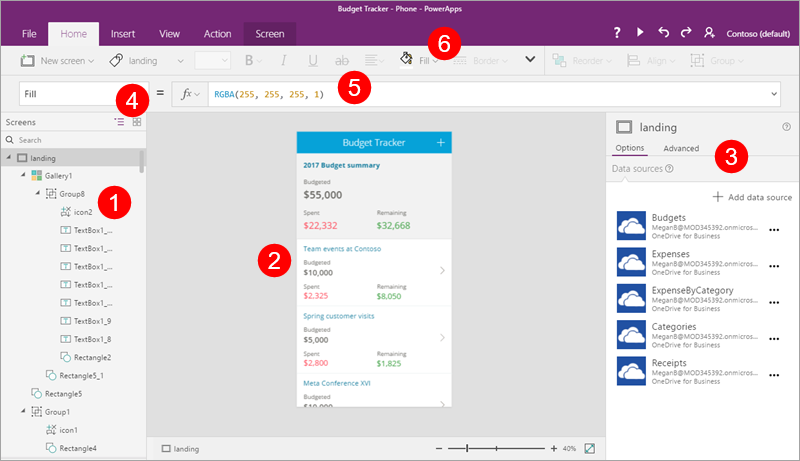
\includegraphics[width=\linewidth]{powerapps-studio.png}
    \caption{Overzicht van Power Apps Studio \autocite{MicrosoftDocs2017}}
    \label{fig:pastudio}
\end{figure}

\subsection{Recente Wijzigingen}

De Test studio valt hierbij (Zie boven). % TODO: datum zetten + een verwijzing

De AI Builder is in publieke preview sinds 10 juni 2019. Dit maakt het mogelijk om AI te gebruiken in Power Apps met minimale technische kennis.\\
Een voorbeeld van het typische verloop: Een AI model type kiezen $\rightarrow$ Data verbinden (uit CDS) $\rightarrow$ AI model aanpassen naar noden (data filteren, scheduling) $\rightarrow$ AI model trainen (gebeurt automatisch) $\rightarrow$ De inzichten van het AI model gebruiken doorheen het Power Platform.\\
Wat AI modellen betreft zijn er enkele keuzes: enerzijds kan er aan aangepast model gebruikt gemaakt worden (voorspelling, form processing, object detectie, text classificatie), anderzijds kan geopteerd worden voor een voorgebouwd. In dat geval is er geen data nodig, het is gebouwd (en getraind) door Microsoft. Mogelijke keuzes zijn: Business card lezer, sleutel zin extractor, taal detectie, text herkenning, gevoelsanalyse. \autocite{MicrosoftDocs2019e}

% TODO: iets over teams wijzigingen/integratie?

\subsection{Pricing, Licencing}

\begin{itemize}
    \item Power Apps voor Office 365.
    \item Plan 1
    \item Plan 2
    \item Power Apps for Dynamics.
\end{itemize} \autocite{Pohl2019}

Elke entry in de lijst heeft meer functionaliteit dan de voorgaande.\\
In Power Apps for office is het enkel mogelijk Canvas apps te maken. Het aantal connectors is beperkt. De on-premise connectors bijvoorbeeld zijn niet aanwezig.

\subsection{Uitbreidingsmogelijkheden}

Power Apps studio is bedoelt als no code omgeving gefocust op business gebruikers. Binnen deze ui is er geen optie om aangepaste code te gebruiken. De enige manier om dit mogelijk te maken is via Custom API's, Azure functions of Azure API apps \footnote{Volgens het antwoord van een Microsoft medewerker op het Power App forum: https://powerusers.microsoft.com/t5/Power-Apps-Ideas/add-your-own-js-in-powerapps-or-call-external-js-file-easily/idi-p/869}.\\
Praktisch gezien is dit mogelijk door een project te maken in Visual studio, een OpenAPI definitie te voorzien. Als deze app in de Azure cloud staan kan deze ook opgeroepen worden vanuit Power Apps \autocite{Jugo2019}

\section{Microsoft Power Platform: Power Automate}

Power automate is een service voor het maken van geautomatiseerde workflows tussen apps en services. Een flow kan gemaakt worden door stappen aaneen te schakelen. Per stap kan een actie of conditie ingesteld worden. In deze condities kunnen data operaties geconfigureerd worden, er zijn ook expressies mogelijk. Naast het zelf bouwen van een flow zijn er sjablonen aanwezig voor gangbare automatisatie cases. Flows kunnen gebruikt worden vanuit Power Apps. \autocite{MicrosoftDocs2019f}

Er zijn vijf soorten flows:
\begin{itemize}
    \item Geautomatiseerde flow: de flow wordt gestart vanuit een bepaalde trigger.
    \item Button flows: de flow wordt manueel gestart. Vaak wordt dit gebruikt vanop een mobiele device.
    \item Scheduled flows: De flow herhaald / op een schema uitvoeren.
    \item Approval flows
    \item UI flows: Een vorm van UI automatisatie, een optie indien er geen API of connector aanwezig is (bijvoorbeeld oudere toepassingen). Voor gebruik met Windows desktop en web applicaties. Momenteel nog in experimentele fase. Het kan gezien worden als een eenvoudige manier om een script te bouwen. De werking is dat de gebruiker een actie/set stappen opneemt, hier wordt dan een aanpasbare flow voor gegenereerd. \autocite{MPA2019}
\end{itemize}

\subsubsection{Beperkingen}

Er is geen aangepaste code of scripting ondersteund.